\documentclass[11pt]{article}
\usepackage{graphicx}
\usepackage{fancyhdr}
% \usepackage{wrapfig}
\usepackage{hyperref}
\usepackage{tabularx}
\usepackage{setspace}
\usepackage{listings}

% math package
\usepackage{amsmath}
\usepackage{amssymb}

% matrix package
\usepackage{nicematrix}

% graph package
\usepackage{tikz}
\usetikzlibrary{positioning}


%\usepackage{yhmath}


% for R style
\usepackage{color}
\definecolor{mGreen}{rgb}{0,0.6,0}
\definecolor{mGray}{rgb}{0.5,0.5,0.5}
\definecolor{mPurple}{rgb}{0.58,0,0.82}
\definecolor{backgroundColour}{rgb}{0.95,0.95,0.92}


\lstdefinestyle{RStyle}{
    backgroundcolor=\color{backgroundColour},   
    commentstyle=\color{mGreen},
    keywordstyle=\color{magenta},
    numberstyle=\tiny\color{mGray},
    stringstyle=\color{mPurple},
    basicstyle=\footnotesize,
    breakatwhitespace=false,
    breaklines=true,
    captionpos=b,
    keepspaces=true,
    numbers=left,
    numbersep=5pt,
    showspaces=false,
    showstringspaces=false,
    showtabs=false,
    tabsize=2,
    language=R
}



\usepackage[spanish]{babel}
\decimalpoint

\newsavebox\CBox
\def\textBF#1{\sbox\CBox{#1}\resizebox{\wd\CBox}{\ht\CBox}{\textbf{#1}}}

\newenvironment{myenv}[1]
  {\begin{spacing}{#1}}
  {\end{spacing}}

\addtolength{\textwidth}{0.2cm}
\setlength{\parskip}{13pt}
\setlength{\parindent}{0.0cm}
\linespread{1.25}

\pagestyle{fancy}
\fancyhf{}
\rhead{TP Final - Cipullo, Bisiach}
\lhead{Probalidad y Estad\'istica}
\rfoot{\vspace{1cm} \thepage}

\renewcommand*\contentsname{\LARGE Índice}

\begin{document}

\begin{titlepage}
    \begin{center}
        \vfill
        \vfill
            \vspace{0.7cm}
            \noindent\textbf{\Huge Trabajo Pr\'actico Final}\par
            \noindent\textbf{\Huge Probabilidad y Estad\'istica}\par
            \vspace{.5cm}
        \vfill
        \noindent \textbf{\huge Alumnos:}\par
        \vspace{.5cm}
        \noindent \textbf{\Large Cipullo, In\'es}\par
        \noindent \textbf{\Large Bisiach, Ezequiel}\par

 
        \vfill
        \large Universidad Nacional de Rosario \par
        \noindent\large 2021
    \end{center}
\end{titlepage}
\par


\section*{Problema 1}

Tenemos un suceso cuya probabilidad de éxito es $p$. Se realizan intentos independientes de este suceso hasta obtener $k$ éxitos consecutivos. 
Definimos el proceso $N_k$ que denota el número de ensayos necesarios para obtener $k$ éxitos consecutivos.

\textbf{a)}

Simulamos 1000 trayectorias del proceso $N_3$, es decir, buscando 3 éxitos consecutivos, con $p = 0.4 < 0.5$. Graficamos en un boxplot los resultados obtenidos.

\begin{center}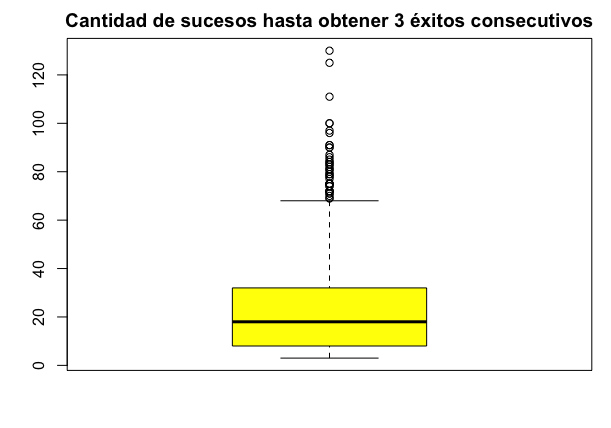
\includegraphics[scale = 0.6]{sucesosEJ1.png}\end{center}

Vemos que la mínima cantidad de sucesos es 3 y, en principio, no tiene límite superior.

Se presenta, además, una tabla con dicho resultado al final del trabajo, que incluye frecuencia absoluta y relativa según la cantidad de sucesos que se obtuvieron en las trayectorias simuladas.

\textbf{b)}

A partir de lo obtenido anteriormente, estimamos la esperanza de $N_3$ haciendo la suma de cada cantidad de sucesos por su respectiva frecuencia relativa, quedando $E(N_3) = 23.255$.

\section*{Problema 2}

Tenemos el proceso $D_n = 2 \cdot I_n - 1$, que representa el cambio de posición de una partícula que se mueve a lo largo de una linea recta con saltos de magnitud 1 en cada momento. Esto se debe a que $D_n$ depende del proceso de Bernoulli $I_n$: ``la señal emitida en el momento $n$ es correcta''. Lo definimos como sigue:

\begin{itemize}
    \item $I_n = 1$ si la señal emitida en el $n$-ésimo momento es correcta
    \item $I_n = 0$ si la señal emitida en el $n$-ésimo momento NO es correcta
\end{itemize}

Tomamos el estado inicial del proceso como $N_0 = 0$, el comienzo de la trayectoria.

\textbf{a)}

Una simulación de 50 pasos de una trayectoria del proceso $D_n$, para un proceso Bernoulli $I_n$ con una probabilidad de éxito $p = 0.75 > 0.7$, es como sigue:

\begin{align*}
    &D_n = [1,-1,1,-1,-1,1,-1,1,1,1,1,1,-1,1,-1,1,1,1,1,1,1,-1,1,1,1,\\
    &1,1,1,1,1,-1,1,1,1,1,1,1,1,1,-1,1,1,1,-1,1,-1,-1,-1,1,-1]
\end{align*}

\textbf{b)}

Definimos otro proceso, $S_n$, proceso estocástico, como la posición de la partícula en el momento n. Notamos que $S_i = D_1 + D_2 + \dots + D_i$, es decir, $S_i$ es la suma acumulada hasta $D_i$.

Del resultado antes expuesto, obtenemos una trayectoria $S_n$ como sigue:

\begin{center}\large\textbf{Simulación de 50 pasos del proceso $S_n$}\end{center}
\vspace{-0.9cm}
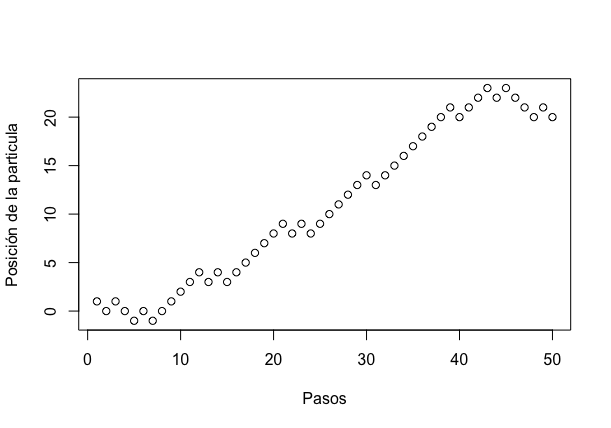
\includegraphics[scale = 0.6]{trayectoriaEJ2.png}

\begin{align*}
    &S_n = [1,0,1,0,-1,0,-1,0,1,2,3,4,3,4,3,4,5,6,7,8,9,8,9,8,9,10,11,12,13,\\
    &14,13,14,15,16,17,18,19,20,21,20,21,22,23,22,23,22,21,20,21,20]
\end{align*}


\section*{Problema 3}

Tenemos un proceso estocástico $N_n$ que representa el estado actual de la apuesta de un jugador luego de $n$ juegos. El estado inicial del proceso es $N_0 = k$, la apuesta inicial. Por cada juego, el jugador puede perder 1 o ganar 1 de su apuesta. Por lo tanto podemos definir el proceso $X_n$ como $X_n = 2 \cdot J_n - 1$, donde $J_n$ es el proceso de Bernoulli que representa: ``el $n$-ésimo juego se ganó'', definido como sigue:

\begin{itemize}
    \item $J_n = 1$ si el $n$-ésimo juego se ganó
    \item $J_n = 0$ si el $n$-ésimo juego NO se ganó
\end{itemize}

Para las simulaciones se toman los valores $k = 10$ y $s = 20$, siendo $p$ variable.

\textbf{a)}

Se realizan simulaciones de la evolución del capital del jugador, para distintos valores de $p$ (probabilidad de éxito de $J_n$), logrando los resultados que siguen:

Para $p = 0.25 < 0.5$,

\begin{center}\large\textbf{Simulación del proceso $N_n$ con $p = 0.25$}\end{center}
\vspace{-0.9cm}
\begin{center}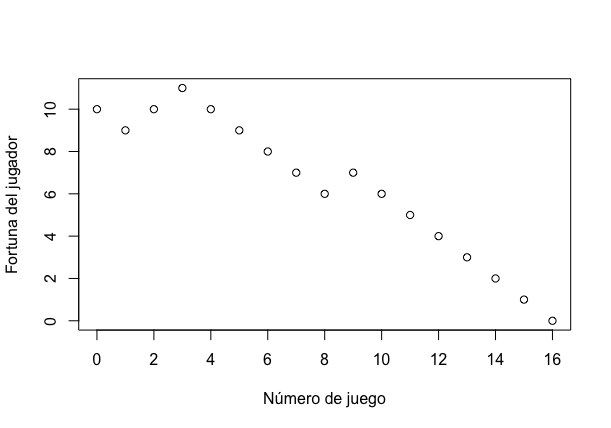
\includegraphics[scale = 0.5]{fortuna1.png}\end{center}

% \begin{align*}
%     [10,9,8,7,6,5,6,7,6,5,4,5,6,5,4,3,4,3,2,1,2,1,2,1,0]
% \end{align*}

Para $p = 0.5$,

\begin{center}\large\textbf{Simulación del proceso $N_n$ con $p = 0.5$}\end{center}
\vspace{-0.9cm}
\begin{center}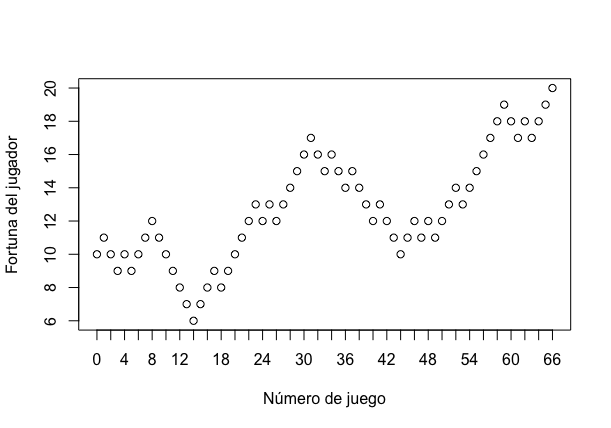
\includegraphics[scale = 0.5]{fortuna2.png}\end{center}

% \begin{align*}
%     &[10,11,12,11,10,11,10,9,8,7,6,5,6,7,8,9,10,9,10,11,12,11,12,13,\\
%     &14,13,14,15,14,15,14,15,16,15,14,13,12,11,12,11,10,9,8,7,6,7,8,\\
%     &9,8,7,8,9,10,11,10,11,12,13,12,13,14,15,16,15,16,17,18,19,18,17,\\
%     &16,15,14,15,16,17,18,17,18,19,20]
% \end{align*}

Para $p = 0.8 > 0.5$,

\begin{center}\large\textbf{Simulación del proceso $N_n$ con $p = 0.8$}\end{center}
\vspace{-0.9cm}
\begin{center}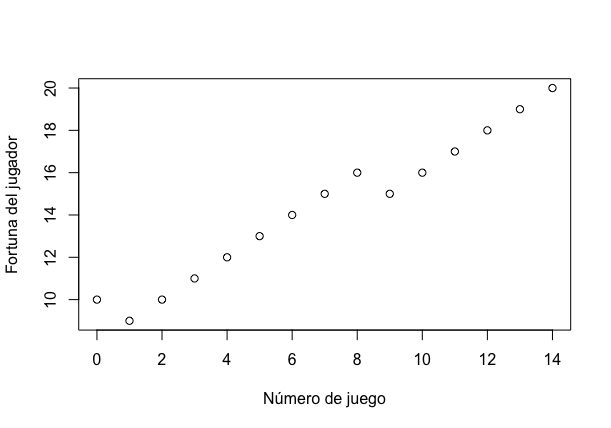
\includegraphics[scale = 0.5]{fortuna3.png}\end{center}

% \begin{align*}
%     [10,11,12,13,12,13,14,15,14,15,16,17,18,19,20]
% \end{align*}


\textbf{b)}

Se simula una cantidad significativa de trayectorias del capital del jugador para luego calcular la probabilidad de ruina (que su fortuna llegue a 0), para los distintos valores de $p$, logrando los resultados que siguen:

Para $p = 0.25 < 0.5$, se obtiene una probabilidad de ruina de 1.

Para $p = 0.5$, se obtiene una probabilidad de ruina de 0.4975.

Para $p = 0.8 > 0.5$, se obtiene una probabilidad de ruina de 0.


\section*{Problema 4}

Se busca medir la efectividad de un algoritmo que opera sobre conjuntos midiendo la cantidad de comparaciones que realiza. Denominamos $M_n$ al número esperado de comparaciones que realiza el algoritmo para un conjunto de $n$ elementos.

\textbf{a)}

Se toma $n = 5$, y luego de hacer 10000 simulaciones del valor de $M_5$, obtenemos las siguientes frecuencias absolutas de las cantidades de comparaciones posibles:

\begin{center}\large\textbf{Frecuencia absoluta del valor de $M_5$ en 10000 simulaciones}\end{center}
\vspace{-0.9cm}
\begin{center}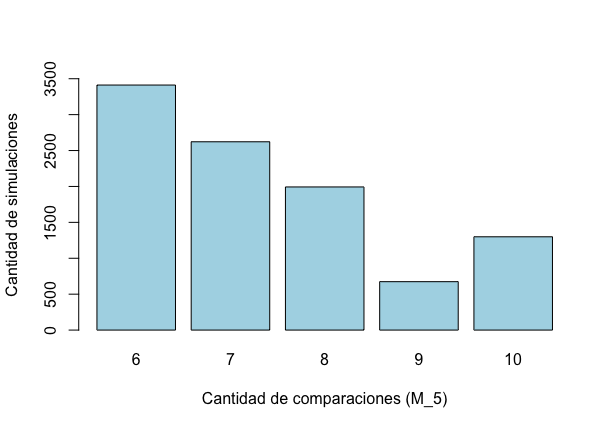
\includegraphics[scale = 0.5]{M_5EJ4.png}\end{center}

, donde la cantidad de comparaciones promedio es 7.3826. Vemos también que el espacio muestral de $M_5$ es $\{6,7,8,9,10\}$.

\textbf{b)}

Análisis formal de la distrubución de probabilidades de la variable aleatoria $M_5$:

Sea una lista $l = [x_1, x_2, x_3, x_4, x_5]$. Se tiene la misma probabilidad de elegir cualquier $x_i, i = 1, \dots ,5$, por lo tanto esta probabilidad es $\frac{1}{n} = \frac{1}{5}$.

Luego de elegir un $x_i$, se realizan $n-1$ comparaciones, en este caso son 4. Dependiendo la elección de $x_i$, se pueden generar diferentes listas a ordenar en el llamado recursivo:

\begin{itemize}
    \item 0 elementos menores a $x_i$ y 4 elementos mayores a $x_i$
    \item 1 elemento menor a $x_i$ y 3 elementos mayores a $x_i$
    \item 2 elementos menores a $x_i$ y 2 elementos mayores a $x_i$
    \item 3 elementos menores a $x_i$ y 1 elemento mayor a $x_i$
    \item 4 elementos menores a $x_i$ y 0 elementos mayores a $_i$
\end{itemize}

Sabemos que ordenar una lista vacía o con un elemento no requiere comparaciones, y que para ordenar una lista de 2 elementos se realiza 1 comparación. Además, ordenar una lista de $m$ elementos tiene el mismo costo, independientemente de sus elementos.

Por lo tanto, llegamos a que hay:

\begin{itemize}
    \item $\frac{2}{5}$ de probabilidad de ordenar una lista de 4 elementos
    \item $\frac{2}{5}$ de probabilidad de ordenar una lista de 3 elementos
    \item $\frac{1}{5}$ de probabilidad de realizar 2 comparaciones
\end{itemize}

Vemos que es necesario conocer la cantidad de comparaciones que se realizan sobre listas de 3 y 4 elementos.

Para listas de 3 elementos, luego de elegir un elemento al azar y realizar 2 comparaciones, hay $\frac{2}{3}$ de probabilidad de que se seleccione el menor o mayor elemento de la lista y por eso realizar 3 comparaciones en total (se le suma solo una comparación a las 2 iniciales), y hay $\frac{1}{3}$ de probabilidad de que se seleccione el elemento central, en cuyo caso no se deberan realizar más comparaciones, debiendo realizar 2 comparaciones en total.

Para listas de 4 elementos, luego de elegir un elemento al azar y realizar 3 comparaciones, hay $\frac{1}{2}$ de probabilidad de que se seleccione el menor o mayor elemento de la lista y que reste ordenar una lista de 3 elementos, y hay $\frac{1}{2}$ de probabilidad de que se haga 1 comparación más por haber elegido alguno de los elementos centrales.

Multiplicando estas probabilidades con lo obtenido para listas de 3 elementos, se obtiene que hay:

\begin{itemize}
    \item $\frac{1}{2}$ de probabilidad de que se realicen 4 comparaciones
    \item $\frac{1}{6}$ de probabilidad de que se realicen 5 comparaciones
    \item $\frac{1}{3}$ de probabilidad de que se realicen 6 comparaciones
\end{itemize}

Juntando todos los calculos realizados, tenemos que la distribución de probabilidad de $M_5$ es:

\begin{itemize}
    \item $\frac{1}{3}$ de probabilidad de que se realicen 6 comparaciones
    \item $\frac{4}{15}$ de probabilidad de que se realicen 7 comparaciones
    \item $\frac{1}{5}$ de probabilidad de que se realicen 8 comparaciones
    \item $\frac{1}{15}$ de probabilidad de que se realicen 9 comparaciones
    \item $\frac{2}{15}$ de probabilidad de que se realicen 10 comparaciones
\end{itemize}

Por último, al ser cantidades númericas, la esperanza se puede calcular como el promedio. Así, llegamos a que $E(M_5) = 7.4$, por lo que concluimos que el resultado obtenido en el apartado anterior es una buena aproximación. También resulta claro que la distribución de probabilidades concuerda con la simulación graficada.


\section*{Problema 5}

Contamos con una red simplificada de 7 páginas. La importancia de cada página se entiende como la probabilidad de que un usuario se encuentre en dicha página luego de un tiempo navegando la red. Esto es lo que mide el algoritmo \verb|PageRank|, para poder asignar un orden de las páginas dentro de la red. Esta probabilidad está medida, entre otras cosas, por la cantidad de enlaces de hipertexto que dirigen al usuario a la página y el peso de estos, que depende de la importancia de la página que lo contiene y cuantos haya.

\textbf{a)}

El comportamiento de visitas de las páginas se puede modelar con la siguiente Cadena de Marcov, y su respectiva matríz de transición en un paso.

% GRAFO
\begin {center}
\begin {tikzpicture}[-latex, auto, node distance = 4 cm and 5cm, on grid, semithick, state/.style = {circle, color = white, draw, black, text = black, minimum width = 1 cm}]
\node[state] (F) {$f$};
\node[state] (E) [above right = of F] {$e$};
\node[state] (B) [above left = of F] {$b$};
\node[state] (G) [right = of F] {$g$};
\node[state] (C) [below left = of F] {$c$};
\node[state] (D) [below right = of F] {$d$};
\node[state] (A) [above = of F] {$a$};
\path (C) edge node[below = 0.15 cm] {$1/2$} (F);
\path (C) edge node[below = 0.15 cm] {$1/2$} (D);
\path (D) edge node[below = 0.15 cm] {$1$} (F);
\path (B) edge node[below = 0.15 cm] {$1/3$} (A);
\path (B) edge node[below = 0.15 cm] {$1/3$} (C);
\path (B) edge [bend right = 15] node[below = 0.15 cm] {$1/3$} (F);
\path (F) edge [bend right = 15] node[below = 0.15 cm] {$1/2$} (B);
\path (F) edge [bend right = 15] node[below = 0.15 cm] {$1/2$} (A);
\path (A) edge [bend right = 15] node[below = 0.15 cm] {$1/2$} (F);
\path (A) edge [bend right = 15] node[below = 0.15 cm] {$1/2$} (E);
\path (E) edge [bend right = 15] node[below = 0.15 cm] {$1/4$} (A);
\path (E) edge [bend right = 15] node[below = 0.15 cm] {$1/4$} (G);
\path (E) edge node[below = 0.15 cm] {$1/4$} (F);
\path (E) edge [bend left = 25] node[below = 0.15 cm] {$1/4$} (D);
\path (G) edge node[below = 0.15 cm] {$1/6$} (D);
\path (G) edge [bend right = 15] node[below = 0.15 cm] {$1/6$} (E);
\path (G) edge node[below = 0.15 cm] {$1/6$} (C);
\path (G) edge node[below = 0.15 cm] {$1/6$} (F);
\path (G) edge [bend left = 25] node[below = 0.15 cm] {$1/6$} (A);
\path (G) edge [bend left = 65] node[below = 0.15 cm] {$1/6$} (B);
\end{tikzpicture}
\end{center}

% MATRIZ
\begin{equation}
    P = \begin{pNiceMatrix}[first-row,first-col]
              & a   & b   & c   & d   & e   & f   & g   \\
            a & 0   & 0   & 0   & 0   & 1/2 & 1/2 & 0   \\
            b & 1/3 & 0   & 1/3 & 0   & 0   & 1/3 & 0   \\
            c & 0   & 0   & 0   & 1/2 & 0   & 1/2 & 0   \\
            d & 0   & 0   & 0   & 0   & 0   & 1   & 0   \\
            e & 1/4 & 0   & 0   & 1/4 & 0   & 1/4 & 1/4 \\
            f & 1/2 & 1/2 & 0   & 0   & 0   & 0   & 0   \\
            g & 1/6 & 1/6 & 1/6 & 1/6 & 1/6 & 1/6 & 0   \\
        \end{pNiceMatrix}
\end{equation}

\textbf{b)}

Se simula una trayectoria de 100 pasos de un usuario en esta red. La página inicial es elegida al azar y todas las páginas tienen igual probabilidad de ser elegidas como tal.

\hspace{-3.6cm}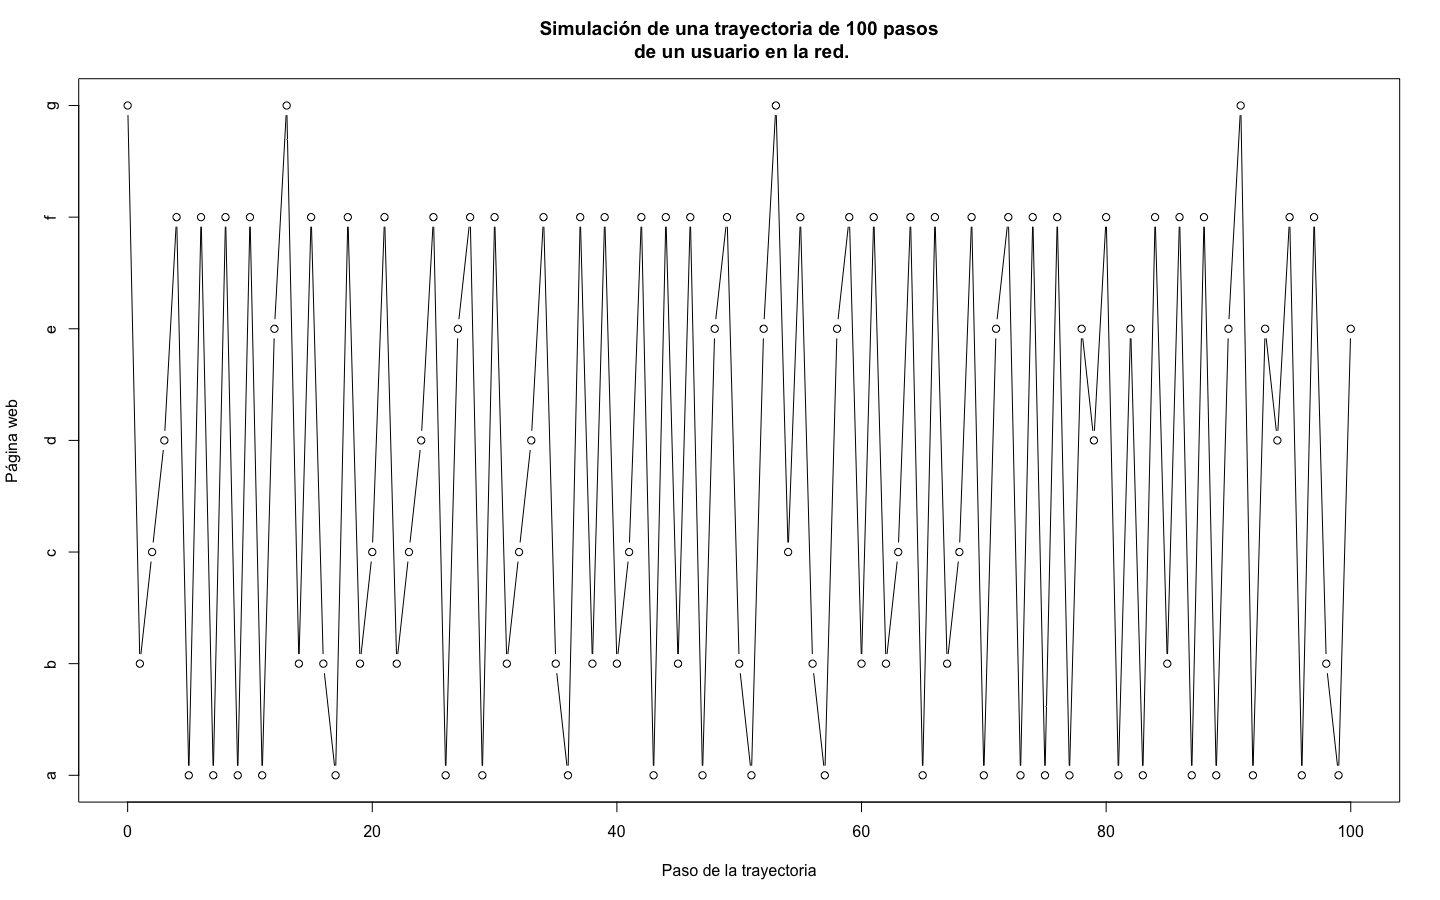
\includegraphics[scale = 0.4]{trayectoriaredEJ5.png}

Para que se visualicen un poco mejor ciertos datos, se muestra también un gráfico de barras sobre la frecuencia absoluta de la cantidad de visitas que recibió cada página web de la red en la trayectoria de 100 pasos del usuario que se simuló.

\begin{center}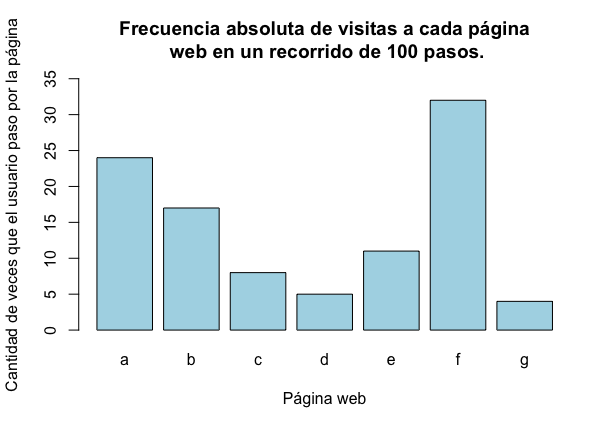
\includegraphics[scale = 0.5]{frecabsEJ5.png}\end{center}

% > cien_pasos
%   [1] 7 2 3 4 6 1 6 1 6 1 6 1 5 7 2 6 2 1 6 2 3 6 2 3 4 6 1 5 6 1 6 2 3 4 6 2 1 6 2 6 2 3 6 1 6 2 6 1 5
%  [50] 6 2 1 5 7 3 6 2 1 5 6 2 6 2 3 6 1 6 2 3 6 1 5 6 1 6 1 6 1 5 4 6 1 5 1 6 2 6 1 6 1 5 7 1 5 4 6 1 6
%  [99] 2 1 5
% > table(cien_pasos)
% cien_pasos
%  1  2  3  4  5  6  7 
% 24 17  8  5 11 32  4 

\textbf{c)}

El rango de página de una página web es la probabilidad a largo plazo de que un usuario se encuentre en dicha página, luego de haber estado navegando en la red. Analiticamente, esto equivale a calcular la distribución invariante $\pi$, la cual podemos asegurar que es única porque la cadena es cerrada, finita, irreducible y aperiódica.

Para ello, planteamos el siguiente sistema lineal de ecuaciones:

\begin{equation}
    \begin{cases}
        \pi_a = \frac{1}{3} \cdot \pi_b + \frac{1}{4} \cdot \pi_e + \frac{1}{2} \cdot \pi_f + \frac{1}{6} \cdot \pi_g \\
        \pi_b = \frac{1}{2} \cdot \pi_f + \frac{1}{6} \cdot \pi_g \\
        \pi_c = \frac{1}{3} \cdot \pi_b + \frac{1}{6} \cdot \pi_g \\
        \pi_d = \frac{1}{2} \cdot \pi_c + \frac{1}{4} \cdot \pi_e + \frac{1}{6} \cdot \pi_g \\
        \pi_e = \frac{1}{2} \cdot \pi_a + \frac{1}{6} \cdot \pi_g \\
        \pi_f = \frac{1}{2} \cdot \pi_a + \frac{1}{3} \cdot \pi_b + \frac{1}{2} \cdot \pi_c + \pi_d + \frac{1}{4} \cdot \pi_e + \frac{1}{6} \cdot \pi_g \\
        \pi_g = \frac{1}{4} \cdot \pi_e \\
        \pi_a + \pi_b + \pi_c + \pi_d + \pi_e + \pi_f + \pi_g = 1 \\
    \end{cases}
\end{equation}

Luego de resolver el sistema (y comparar el resultado con la aproximación de R), el rango de cada página es:

\begin{equation}
    \pi = \begin{pNiceMatrix}[first-row]
        a      & b    & c      & d      & e     & f      & g     \\
        0.2453 & 0.16 & 0.0587 & 0.0667 & 0.128 & 0.3093 & 0.032 \\
    \end{pNiceMatrix}
\end{equation}

\section*{Problema 6}

El evento bajo estudio es el número de vuelos que recibe un aeropuerto a una tasa $\lambda$ aterrizajes/hora.

\textbf{a)}

Con una tasa de 3 aterrizajes por hora de acuerdo a un proceso de Poisson, el aeropuerto recibe vuelos a partir de las 2 am. Para visualizar el comportamiento de dicho proceso por 24 horas, se presenta el siguiente gráfico de la trayectoria obtenida.

\hspace{-1.9cm}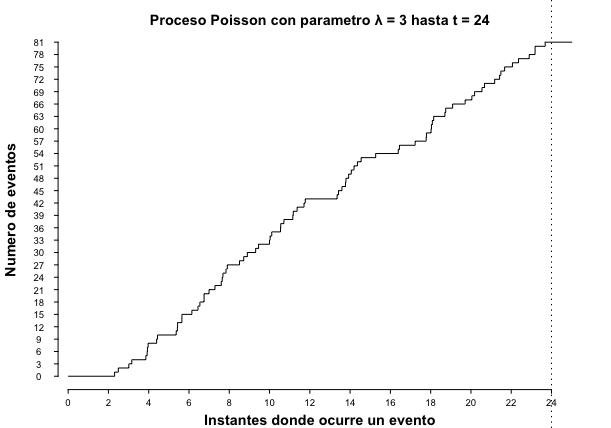
\includegraphics[scale = 0.8]{poissonEJ6.png}

Esta trayectoria se obtiene de la siguiente forma: el número aleatorio de la distribución de Poisson con parámetro $\lambda \cdot t$ retorna la cantidad de eventos que ocurren en el tiempo $t$ en un Proceso de Poisson a una tasa $\lambda$. Luego las probabilidades de que un evento ocurra a un momento determinado es la misma para cada evento, por lo tanto se generan números aleatorios de la distribución uniforme hasta $t$, los cuales serán los instantes en los que ocurre un evento.


\textbf{b)}

Se realiza una simulación del proceso de Poisson antes descripto para un intervalo de tiempo de $T = 1000$ horas. Una vez que se saben los instantes en los que ocurre cada evento, se calculan las diferencias entre cada par de instantes consecutivos, obteniendo así los tiempos entre arribos. De este resultado, surge el siguiente histograma:

\begin{center}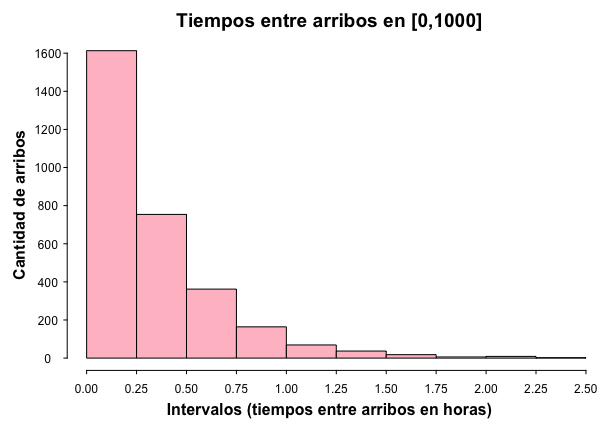
\includegraphics[scale = 0.6]{interarribosEJ6.png}\end{center}

Además, sabemos que el tiempo transcurrido entre dos arribos sucesivos es independiente de los arribos de los que se trate y de los instantes de los arribos previos, y estos tienen una distribución exponencial. Por ello, su esperanza es $\frac{1}{3}$, lo cual concuerda con lo visto en el gráfico.

\section*{Problema 7}

Tenemos un honeypot, cuyos datos son estudiados utilizando cadenas de Marcov. Se obtienen los datos desde una base de datos central y se observan ataques contra cuatro puertos de computadoras (80, 135, 139 y 445) durante un año. Los estados de la cadena de Markov son los cuatro puertos y se incluye un nodo indicando que ningún puerto está siendo atacado (NA). Los datos se monitorean semanalmente y el puerto más atacado durante la semana es guardado. La matríz de transición para la cadena estimada para los ataques semanales es:

\begin{equation}
    P = \begin{pNiceMatrix}[first-row,first-col]
                & 80   & 135  & 139  & 445  & NA   \\
            80  & 0    & 0    & 0    & 0    & 1    \\
            135 & 0    & 8/13 & 3/13 & 1/13 & 1/13 \\
            139 & 1/16 & 3/16 & 3/8  & 1/4  & 1/8  \\
            445 & 0    & 1/11 & 4/11 & 5/11 & 1/11 \\
            NA  & 0    & 1/8  & 1/2  & 1/8  & 1/4  \\
        \end{pNiceMatrix}
\end{equation}

con distribución inicial $\pi_0 = (0,0,0,0,1)$.

\textbf{a)}

$P$ es la matríz de transición en un paso (una semana) y $\pi_0$ la distribución inicial, por lo tanto $\pi_0 * P^3$ será la distribución de probabilidad de que los puertos sean atacados luego de 3 semanas.

\begin{equation}
    \pi_0 * P^3 = \begin{pNiceMatrix}[first-row]
        80         & 135       & 139       & 445      & NA        \\
        0.02417504 & 0.2422698 & 0.3482356 & 0.232574 & 0.1527455 \\
    \end{pNiceMatrix}
\end{equation}

Para estar seguros de que corresponde a una distribución de probabilidades, notamos que su suma da 1.

Concluimos, entonces, que el puerto 80 es el de menor probabilidad de ser atacado y el puerto 139 es el de mayor probabilidad de ser atacado, quedando los puertos 135 y 445 en el medio.

\textbf{b)}

Tenemos la cadena de Marcov definida por la matríz $P$ de transición en un paso. Como $E = \{80, 135, 139, 445, NA\}$ es un conjunto cerrado, irreducible y finito, deducimos que sus elemento son estados positivamente recurrentes. 
Además, tenemos que $P^3(80,80) = 0.03125 > 0$, $P(135,135) = 8/13 > 0$, $P(139,139) = 3/8 > 0$, $P(445,445) = 5/11 > 0$ y $P(NA,NA) = 1/4 > 0$. Luego todos los estados son aperiódicos.

Por lo tanto, tenemos una cadena de Marcov cerrada, irreducible, finita, recurrente y aperiódica, es decir, tenemos una cadena de Marcov ergódica.

Como $\forall\ j \in E,\ j$ es un estado positivamente recurrente y aperiódico, tenemos que 
$$\forall\ i \in E, \lim_{n \to \infty} P^n(i,j) = F(i,j) \cdot \lim_{n \to \infty} P^n(j,j)$$

Además, sabemos que si $a$ y $b$ son ambos estados recurrentes y ambos pertenecen al mismo cerrado, se tiene $F(a,b)=1$.

Por lo tanto, $\forall\ i \in E, \lim_{n \to \infty} P^n(i,j) = \lim_{n \to \infty} P^n(j,j)$.

Como la cadena de Marcov es irreducible, finita y aperiódica, su distribución invariante ($\pi$) es única y cumple que:

\begin{itemize}
    \item $\pi \cdot P = \pi$
    \item $\sum_{i \in E} \pi_i = 1$
    \item $\pi_j = \lim_{n \to \infty} P^n(i,j)\ \forall\ i,j \in E$
\end{itemize}

Planteamos el correspondiente sistema lineal de ecuaciones para obtenerla.

\begin{equation}
    \begin{cases}
        \pi_{80} = \frac{1}{16} \cdot \pi_{139} \\
        \pi_{135} = \frac{8}{13} \cdot \pi_{135} + \frac{3}{16} \cdot \pi_{139} + \frac{1}{11} \cdot \pi_{445} + \frac{1}{8} \cdot \pi_{NA} \\
        \pi_{139} = \frac{3}{13} \cdot \pi_{135} + \frac{3}{8} \cdot \pi_{139} + \frac{4}{11} \cdot \pi_{445} + \frac{1}{2} \cdot \pi_{NA} \\
        \pi_{445} = \frac{1}{13} \cdot \pi_{135} + \frac{1}{4} \cdot \pi_{139} + \frac{5}{11} \cdot \pi_{445} + \frac{1}{8} \cdot \pi_{NA} \\
        \pi_{NA} = \pi_{80} + \frac{1}{13} \cdot \pi_{135} + \frac{1}{8} \cdot \pi_{139} + \frac{1}{11} \cdot \pi_{445} + \frac{1}{4} \cdot \pi_{NA} \\
        \pi_{80} + \pi_{135} + \pi_{139} + \pi_{445} + \pi_{NA} = 1 \\
    \end{cases}
\end{equation}

Luego de resolverlo, obtenemos la distribución límite de los puertos atacados:

\begin{equation}
    \pi = \begin{pNiceMatrix}[first-row]
        80     & 135    & 139    & 445    & NA     \\
        0.0215 & 0.2669 & 0.3435 & 0.2273 & 0.1408 \\
    \end{pNiceMatrix}
\end{equation}


\section*{Anexo}

Tabla correspondiente al apartado a del problema 1.

\begin{center}
    \large\textbf{Cantidad de sucesos hasta obtener 3 éxitos consecutivos}
    
    \begin{tabularx} {0.7\textwidth}{ 
        | >{\raggedright\arraybackslash}X 
        | >{\raggedleft\arraybackslash}X 
        | >{\raggedleft\arraybackslash}X | }
        \hline
        \textbf{Cantidad de sucesos} & \textbf{Frecuencia absoluta} & \textbf{Frecuencia relativa} \\
        \hline
        3 & 71 & 0.071 \\
        \hline
        4 & 44 & 0.044 \\
        \hline
        5 & 36 & 0.036 \\
        \hline
        6 & 35 & 0.035 \\
        \hline
        7 & 41 & 0.041 \\
        \hline
        8 & 31 & 0.031 \\
        \hline
        9 & 29 & 0.029 \\
        \hline
        10 & 43 & 0.043 \\
        \hline
        11 & 29 & 0.029 \\
        \hline
        12 & 24 & 0.024 \\
        \hline
        13 & 26 & 0.026 \\
        \hline
        14 & 22 & 0.022 \\
        \hline
        15 & 29 & 0.029 \\
        \hline
        16 & 21 & 0.021 \\
        \hline
        17 & 16 & 0.016 \\
        \hline
        18 & 20 & 0.020 \\
        \hline
        19 & 26 & 0.026 \\
        \hline
        20 & 21 & 0.021 \\
        \hline
        21 & 20 & 0.020 \\
        \hline
        22 & 21 & 0.021 \\
        \hline
        23 & 26 & 0.026 \\
        \hline
        24 & 11 & 0.011 \\
        \hline
        25 & 19 & 0.019 \\
        \hline
        26 & 13 & 0.013 \\
        \hline
        27 & 17 & 0.017 \\
        \hline
        28 & 19 & 0.019 \\
        \hline
        29 & 13 & 0.013 \\
        \hline
        30 & 12 & 0.012 \\
        \hline
        31 & 12 & 0.012 \\
        \hline
        32 & 6 & 0.006 \\
        \hline
        33 & 10 & 0.010 \\
        \hline
        34 & 15 & 0.015 \\
        \hline
        35 & 8 & 0.008 \\
        \hline
    \end{tabularx}    
    \begin{tabularx} {0.7\textwidth}{ 
        | >{\raggedright\arraybackslash}X 
        | >{\raggedleft\arraybackslash}X 
        | >{\raggedleft\arraybackslash}X | }
        \hline    
        36 & 7 & 0.007 \\
        \hline
        37 & 11 & 0.011 \\
        \hline
        38 & 6 & 0.006 \\
        \hline
        39 & 5 & 0.005 \\
        \hline
        40 & 10 & 0.010 \\
        \hline
        41 & 8 & 0.008 \\
        \hline
        42 & 10 & 0.010 \\
        \hline
        43 & 11 & 0.011 \\
        \hline
        44 & 14 & 0.014 \\
        \hline
        45 & 8 & 0.008 \\
        \hline
        46 & 3 & 0.003 \\
        \hline
        47 & 4 & 0.004 \\
        \hline
        48 & 6 & 0.006 \\
        \hline
        49 & 6 & 0.006 \\
        \hline
        50 & 6 & 0.006 \\
        \hline
        51 & 9 & 0.009 \\
        \hline
        52 & 4 & 0.004 \\
        \hline
        53 & 3 & 0.003 \\
        \hline
        54 & 4 & 0.004 \\
        \hline
        55 & 3 & 0.003 \\
        \hline
        56 & 4 & 0.004 \\
        \hline
        57 & 3 & 0.003 \\
        \hline
        58 & 3 & 0.003 \\
        \hline
        59 & 4 & 0.004 \\
        \hline
        60 & 1 & 0.001 \\
        \hline
        61 & 2 & 0.002 \\
        \hline
        63 & 4 & 0.004 \\
        \hline
        64 & 2 & 0.002 \\
        \hline
        65 & 4 & 0.004 \\
        \hline
        66 & 2 & 0.002 \\
        \hline
        67 & 3 & 0.003 \\
        \hline
        68 & 1 & 0.001 \\
        \hline
        69 & 2 & 0.002 \\
        \hline
        70 & 1 & 0.001 \\
        \hline
        71 & 2 & 0.002 \\
        \hline
    \end{tabularx}    
    \begin{tabularx} {0.7\textwidth}{ 
        | >{\raggedright\arraybackslash}X 
        | >{\raggedleft\arraybackslash}X 
        | >{\raggedleft\arraybackslash}X | }
        \hline
        72 & 4 & 0.004 \\
        \hline
        74 & 2 & 0.002 \\
        \hline
        75 & 5 & 0.005 \\
        \hline
        77 & 1 & 0.001 \\
        \hline
        78 & 2 & 0.002 \\
        \hline
        79 & 2 & 0.002 \\
        \hline
        80 & 1 & 0.001 \\
        \hline
        81 & 2 & 0.002 \\
        \hline
        82 & 1 & 0.001 \\
        \hline
        83 & 2 & 0.002 \\
        \hline
        84 & 2 & 0.002 \\
        \hline
        85 & 1 & 0.001 \\
        \hline
        86 & 1 & 0.001 \\
        \hline
        87 & 1 & 0.001 \\
        \hline
        90 & 2 & 0.002 \\
        \hline
        91 & 2 & 0.002 \\
        \hline
        96 & 1 & 0.001 \\
        \hline
        97 & 1 & 0.001 \\
        \hline
        100 & 2 & 0.002 \\
        \hline
        111 & 1 & 0.001 \\
        \hline
        125 & 1 & 0.001 \\
        \hline
        130 & 1 & 0.001 \\
        \hline \hline
        Total: & 1000 & 1\\
        \hline
    \end{tabularx}
\end{center}




\end{document} 